\documentclass[conference]{IEEEtran}
\IEEEoverridecommandlockouts
% The preceding line is only needed to identify funding in the first footnote. If that is unneeded, please comment it out.
\usepackage{cite}
\usepackage{amsmath,amssymb,amsfonts}
\usepackage{algorithmic}
\usepackage{graphicx}
\usepackage{textcomp}
\usepackage{xcolor}
\usepackage{enumerate}
\usepackage{booktabs}
\usepackage{float}
\usepackage{hyperref}
\usepackage{subfigure}
\usepackage{subcaption}
\def\BibTeX{{\rm B\kern-.05em{\sc i\kern-.025em b}\kern-.08em
    T\kern-.1667em\lower.7ex\hbox{E}\kern-.125emX}}
\begin{document}

\title{G01 - Multi-Label Plant Species Prediction with
Convolutional Neuron Network and Vision Transformer Models\\
}
\author{\IEEEauthorblockN{Patrick Foster}
\IEEEauthorblockA{\textit{University of Virginia} \\
\textit{School of Data Science}\\
Norfolk, Virginia \\
ezq9qu@virginia.edu}
\and
\IEEEauthorblockN{Hai Liu}
\IEEEauthorblockA{\textit{University of Virginia} \\
\textit{School of Data Science}\\
Charlottesville, Virginia \\
hl9h@virginia.edu}
\and
\IEEEauthorblockN{John Michael Epperson}
\IEEEauthorblockA{\textit{University of Virginia} \\
\textit{School of Data Science}\\
Charlottesville, Virginia \\
jme3qd@virginia.edu}
}

\maketitle

\begin{abstract}
This project aims at the PlantCLEF2025 Kaggle/LifeCLEF challenge on multi-species plant identification in unlabeled vegetation quadrat images. We describe a pipeline for the zero-shot multi-species plant identification task starting from a ResNet-50 Convolutional Neural Network (CNN) model as a baseline and a fine-tuned pretrained Vision Transformer (ViT) model. We explored combinations of high-resolution image tiling methods and various prediction aggregation strategies in order to improve the model prediction performance. Our code and work description are available on GitHub (\url{https://github.com/jme-sds/multi_plant_id}).
\end{abstract}


\begin{IEEEkeywords}
Kaggle Challenge, PlantCLEF2025, Vision Transformer, Multi-label Classification, Transfer Learning
\end{IEEEkeywords}

\section{Introduction}
    Vegetation plot inventories are essential tools in ecological research, providing standardized methods for assessing biodiversity, monitoring long-term ecological change, and supporting evidence-based conservation efforts. These inventories typically consist of multiple quadrats—small sampling plots of roughly 0.5 m²—within which botanists identify all plant species and record measurements such as biomass, ecological scores, or the proportion of area occupied by each species \cite{goeau2024overviewplantclef2024multispecies}.
    
    Automating this process with artificial intelligence could greatly enhance efficiency and scalability, enabling broader ecological surveys while reducing dependence on manual annotation by experts. Yet, developing robust AI models for multi-species plant identification remains a major challenge and proposes a \textbf{big gap}. This is because, ideally, training would require large datasets of quadrat images annotated with all species present, but such data are extremely costly to obtain due to the vast species diversity within a single flora. In contrast, extensive repositories of single-plant images already exist and can be used to train powerful single-species classifiers \cite{goeau2024overviewplantclef2024multispecies}\cite{martellucci2025overviewplantclef2025multispecies}.
    
    The PlantCLEF2025 challenge aims to bridge this gap by evaluating models that predict all species present in quadrat images using training data composed of only single-label images of individual plants (Figure 1). This task is framed as a \textbf{multi-label image classification problem} and is complicated by a substantial domain shift between training and test data—moving from isolated, single-plant images to complex, high-resolution vegetation scenes containing multiple species.

    Machine learning has become a dominant paradigm for image analysis, such as object classification/identification, with convolutional neural networks (CNNs) historically forming the backbone of most approaches. Recent advancements in Vision Transformers (ViTs) have achieved equivalent or even state-of-the-art performance in this domain.  

    In the PlantCLEF2024 competition, most of the teams have chosen to use the pre-trained ViTD2PC24All model due to its state-of-the-art ViT architecture, self-supervised pretraining algorithm, and the fine-tuned full model weights.  Also, all of the top three teams have chosen a tiling inference pipeline that makes predictions on sub-images (or "tiles") of a high resolution multi-species test image, although detailed tiling strategies varied among teams\cite{goeau2024overviewplantclef2024multispecies}. For the analysis of each tile and subsequent prediction aggregation over all of the tiles, methods like Segment-Anything Model (SAM) for false positive removal\cite{foy2024-1stplace}, embedding extraction\cite{gustineli2024-3rdplace}, and Bayesian Model Averaging (BMA) for prediction aggregation\cite{Chulif2024-2ndplace}, seemed to have the most contributions to the model performances .

Recent results from the \textbf{PlantCLEF2025} challenge highlight practical innovations in this space. The highest-scoring submission by TheHeartOfNoise leveraged JPEG recompression as a regularization 
technique to mitigate distribution shifts between training and test data, achieving an F1 score of 0.35 on the multi-label species classification task using a pretrained DINOv2 vision transformer backbone 
\cite{martellucci2025overviewplantclef2025multispecies}. Similarly, Herasimchyk et al. enhanced DINOv2 by adding multi-head attention mechanisms to enable simultaneous genus and species classification \cite{herasimchyk2025multilabelplantspeciesprediction}. Notably, among the 
top ten submissions, only one team employed a CNN architecture for species-level prediction, underscoring the growing dominance of transformer-based models in this application.

To leverage deep learning techniques, we aim to create a FAISS index and, by training a ViT classification head (DINOV2) trained on unlabeled quadrats, significantly improve results over untrained counterparts. We start by performing ablations (tiling, pooling, voting) on a baseline ResNet model and then apply the lessons learned to further Vision Transformer Models. 


\section{Dataset}

The PLANTCLEF2025 Challenge provided datasets needed for both training and testing. 

The training dataset is composed of observations of individual plants. The data specifically are images of 7.8 thousand plant species from across southern Europe. The data consists of 1.4 million images with labels. There is also a complementary training set used to help models better adapt to multi-species vegetation quadrat images. The data consists of a large number of unannotated pseudo-quadrat images, ground vegetation images similar to vertical quadrats, but not covering the precise 50cm x 50cm areas. This dataset is useful for self-supervised pre-training steps before moving on to labeled individual plant images. Specifically, the data consists of 212,782 images derived from the LUCAS Cover-Photos 2006-2018 collection.\cite{essd-14-4463-2022} \cite{martellucci2025overviewplantclef2025multispecies}

\textbf{Single plant training set:} 

%    Training set - Min side size - 800px [281GB]
%(\url{https://lab.plantnet.org/LifeCLEF/PlantCLEF2024/single_plant_training_data/#PlantCLEF2024singleplanttrainingdata.tar})
    Training set - Max side size - 800px [160GB]
(\url{https://lab.plantnet.org/LifeCLEF/PlantCLEF2024/single_plant_training_data/PlantCLEF2024singleplanttrainingdata_800_max_side_size.tar})

\textbf{Complementary training set: high-resolution pseudo quadrat images without labels:}
 (\url{https://essd.copernicus.org/articles/14/4463/2022/} \cite{essd-14-4463-2022}
%    Training metadata
%(\url{https://lab.plantnet.org/LifeCLEF/PlantCLEF2024/single_plant_training_data/PlantCLEF2024singleplanttrainingdata.csv})

\begin{figure}[h!]
    \centering
    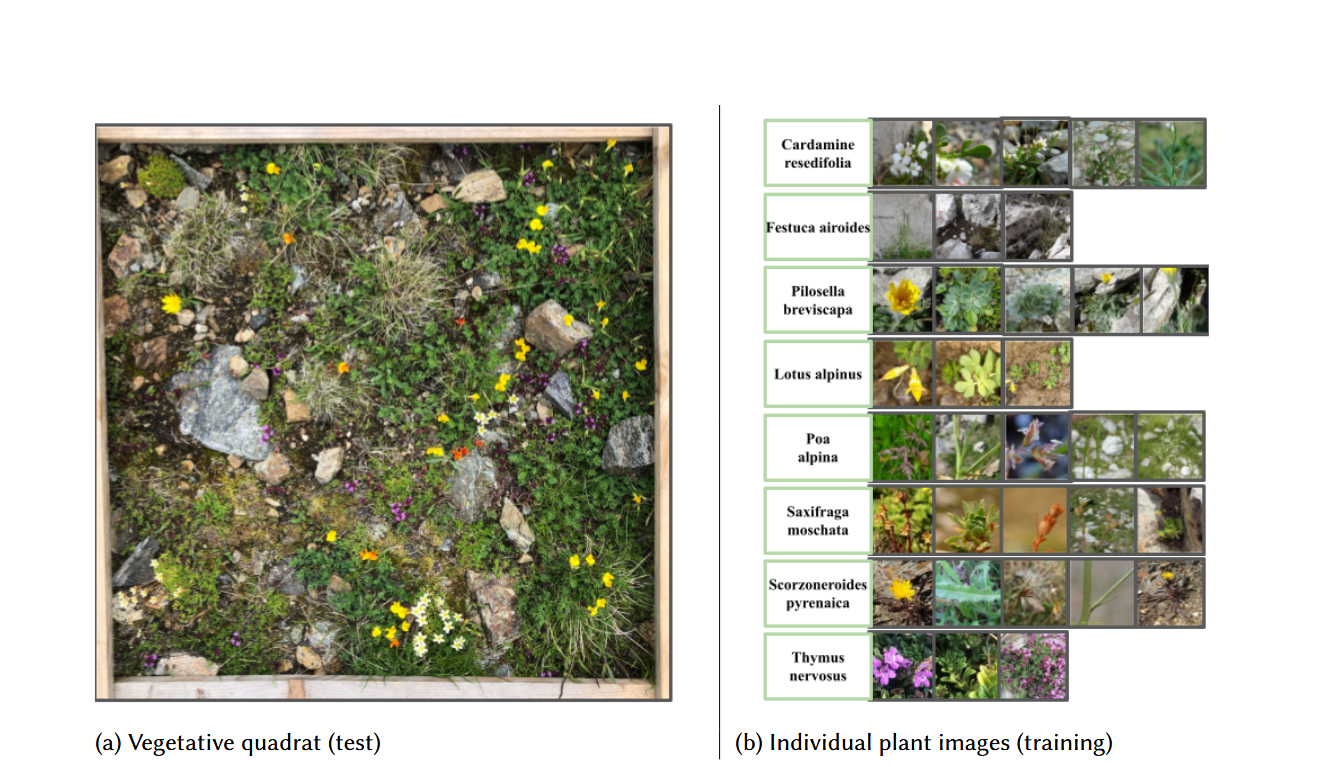
\includegraphics[width=1\linewidth]{Screenshot 2025-10-25 133647.png}
    \caption{Examples}
\end{figure}

The test set is a compilation of several image datasets of plots in different floristic contexts, including Pyrenean and Mediterranean floras. The images can differ from observation to observation; for example, whether wooden frames or measuring tape are used to delimit the plot, and the angles of view relative to the ground. Additionally, the quality of the images may vary depending on the weather, which can result in more or less pronounced shadows, blurry areas, etc. \cite{martellucci2025overviewplantclef2025multispecies}

\textbf{Test set: }

vegetation quadrat images
(\url{https://lab.plantnet.org/LifeCLEF/PlantCLEF2024/vegetation_plot_test_data/PlantCLEF2024test.tar})

\section{Proposed Method}

We propose to leverage the rich embedding space/feature representations that are learned/extracted by the fine-tuned and pretrained ViT model (ViTD2PC24All) for the downstream classification task. Using a tiling approach that divides each test image into a grid of \textit{N} × \textit{M} tiles, followed by label classification for each tile, we can greatly preserve the image quality/resolution, providing the model with usable information to capture objects. With appropriate post-processing steps, we hope our model to achieve domain-expert performance on the zero-shot multi-label classification task.

The complete pipeline comprises the following steps:
\begin{enumerate}
    \item \textbf{Image preprocessing}: Tiling of test images into $\textit{N} \times \textit{M}$ tiles ($N,M\in \{3,4,5,6,7,8,9\}$), followed by adaptive upscaling/downscaling to ensure consistent tile dimensions (as shown in Figure 2);
    \item \textbf{Feature extraction}: Extract the $[\text{CLS}]$ token embeddings for each single-plant training image and build a FAISS Index bank with these labeled embeddings, acting as a ”Knowledge Base” for retrieval. Extract the $[\text{CLS}]$ token embeddings for each tile using the \textit{ViTD2PC24All} model to be used as query to search the "Knowledge Base";
    \item \textbf{Tile-level classification}: Application of multi-label classification inference to each tile with ResNet50 baseline. Application of FAISS Index search with each of the unlabeled quadrat tile embeddings as query to retrieve the \textit{k} Nearest Neighbors (\textit{k}-NN) as predictions;
    \item \textbf{Multi-label aggregation}: Fusion of tile-level predictions via a configurable inference pipeline (\textit{i.e.}, \textbf{voting and pooling}) to produce final multi-label outputs;
    \item \textbf{Ablation study}: We hypothesize that \textbf{tiling} can greatly preserve the image quality of plant objects in the quadrat images and allow models to effectively capture both small and large plant objects, \textbf{voting} with an optimal threshold can effectively remove false positives and increase precision, and that \textbf{pooling} can effectively mitigate the potential issues of decreased recall (missed true positives by voting) and plants being split at tile boundaries. In addition, \textbf{fine tuning} the \textit{ViTD2PC24All} model with the complementary pseudo-quadrat dataset can provide for domain adaptation before using it on the test images. 
\end{enumerate}

\begin{figure}[H]
    \centering
    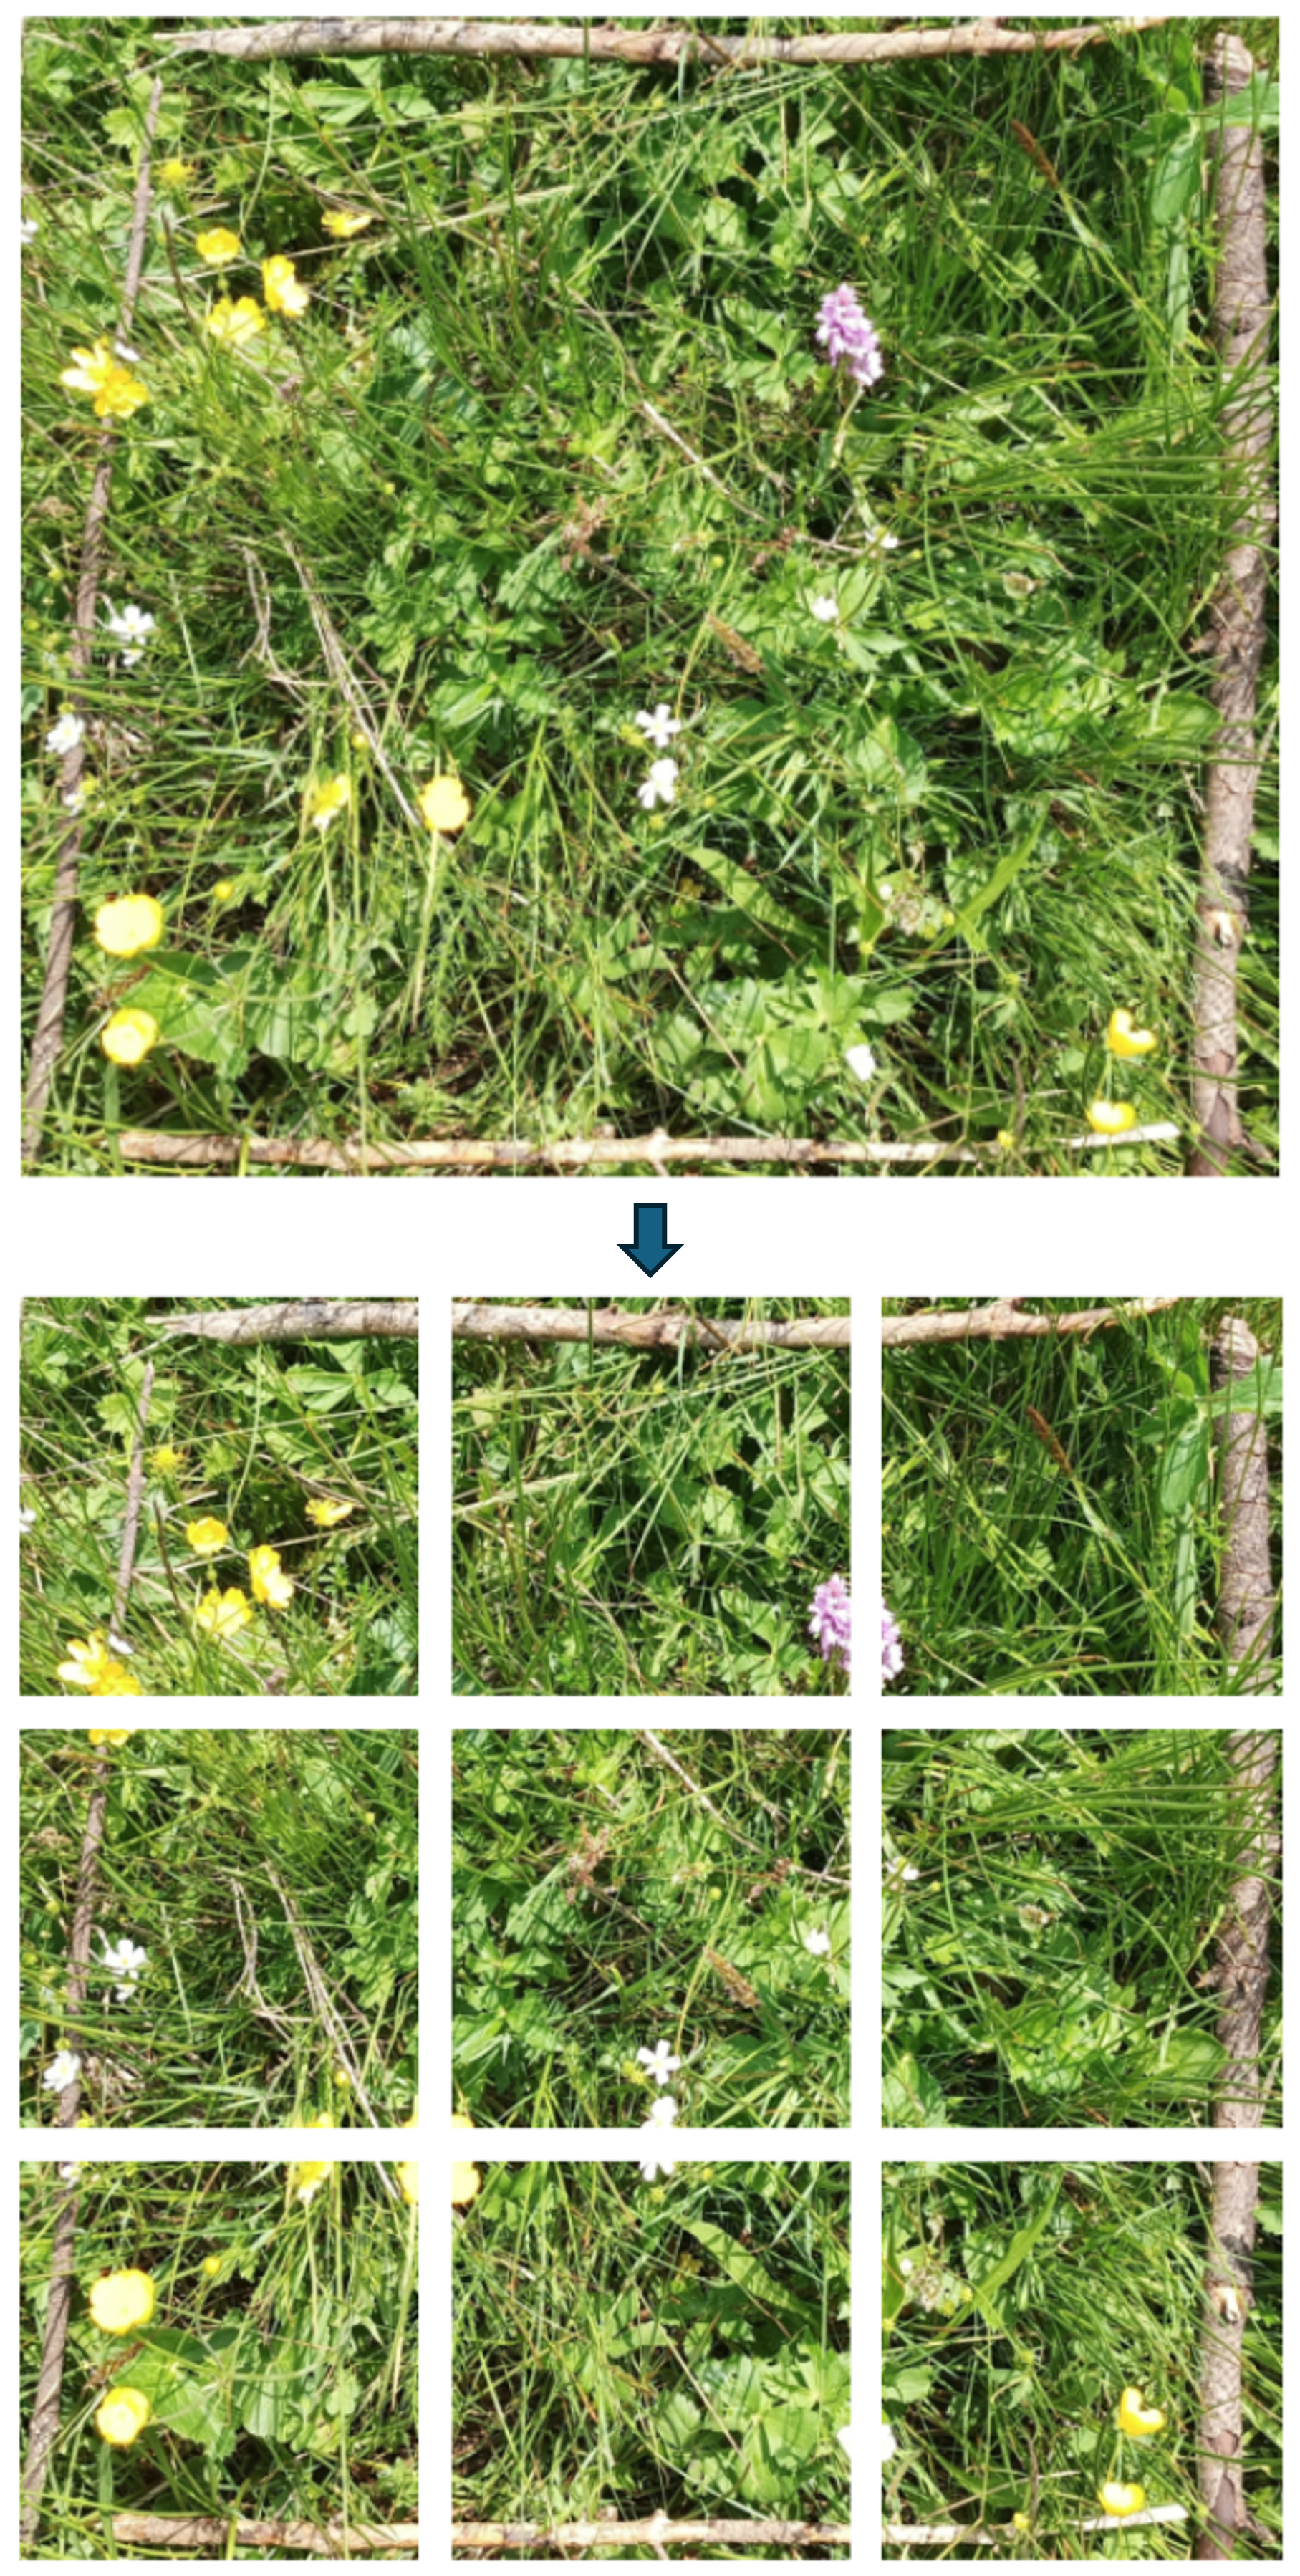
\includegraphics[width=0.6\linewidth]{quadrat_tiling.png}
    \caption{An example of the 3x3 tiling strategy on a quadrat image}
\end{figure}

\section{Experiments}
The goal of the PLANTCLEF2025 challenge was to predict the presence of one or more plant species in each high-resolution quadrat image, selecting from thousands of possible species. Quadrat images typically cover 50×50 cm, meaning that while multiple species may be present, it is uncommon to have dozens of species simultaneously.

To rank the submissions, we use an F1 score-based metric, designed to balance recall and precision. This ensures that models do not over-predict species (leading to low precision) nor under-predict species (resulting in low recall).

 For this project, we use the macro-averaged F1 score per sample, which is particularly suited for multi-label classification problems. This approach ensures a fair evaluation of each image independently, rather than being influenced by class distribution. This also allows us to compare our results with the published teams' scores.

The  test set consists of several quadrat images, each representing a sample of a specific area within a selected site (a 5m*1m area in Pyrenees for example). This surveying process, commonly known in ecology literature as a 'transect', is designed to assess biodiversity across a broad section of the site. To mitigate bias from over-sampled areas, the macro-averaged F1 scores are first computed across all the different transects in the test set and then averaged to return the final score. 


The final score is then computed as:

$$\frac{1}{N} \sum_{i=1}^{N}(\frac{1}{T_i}\sum_{j=1}^{T_i}{\text{F}}1^j)$$

where: 
\begin{itemize}
    \item $N$ is the total number of transects.
    \item $T_i$ is the number of quadrats in the transect
    \item $\frac{1}{T_i}\sum_{j=1}^{T_i}{\text{F}}1^j$ is the macro-averaged F1-score per sample of transect
    \item ${\text{F}}1^j$ is the F1 score for test image , calculated as:
\end{itemize}

    $${\text{F}}1^j = \frac{2 \cdot \text{Precision}_j \cdot \text{Recall}_j}{\text{Precision}_j+ \text{Recall}_j}$$

where for each test image $j$:  
\begin{itemize}
    \item $TP_j \mathbf{(True Positives)}$: number of plant species correctly predicted.
    \item $FP_j \mathbf{(False Positives)}$: number of plant species incorrectly predicted.
    \item $FN_j\mathbf{(False Negatives)}$: number of plant species missed.
\end{itemize}
\cite{martellucci2025overviewplantclef2025multispecies}

%We also quantify key computational metrics for our vision transformer implementation, including model parameter count, floating-point operations (FLOPS), inference latency, and memory footprint. These metrics enable rigorous comparative analysis against the pre-trained DINOv2 architecture (a standard vision transformer variant), providing insights into the computational efficiency, scalability, and real-world applicability of our approach for multi-label plant species classification from quadrat imagery.

\subsection{Data Loading}
In order to load the various datasets, different strategies were used. First, for the single plant dataset, the images were centered, then resized, and finally transformed into a tensor data type. This allows for all the images of plants to be used for training our baseline resnet and DinoV2 models.

The quadrat images were a bit more challenging to deal with. It starts the same way, by centering and resizing so that all images are the same size. However, a grid is used to split the full image into tiles. This way, by running KNN on each different tile, the votes can be pooled together, and we have more knowledge than with a single tiling strategy (full image).

\subsection{ResNet50 Baseline}
To compare the performance between CNN-based and ViT-based SOTA models, we chose ResNet50 (39.5M parameters), a top of the line CNN model, as our baseline model. We first replaced the last feed forward layer with a multi-label classification head and trained only the multi-label classification head for 15 epochs with the full single-plant training image data set. Then, we unfroze most of the layers, making 96.3\% of the total model parameters trainable, and fine tuned the model with the same training data set for another 20 epochs.

\begin{figure}[H]
    \centering
    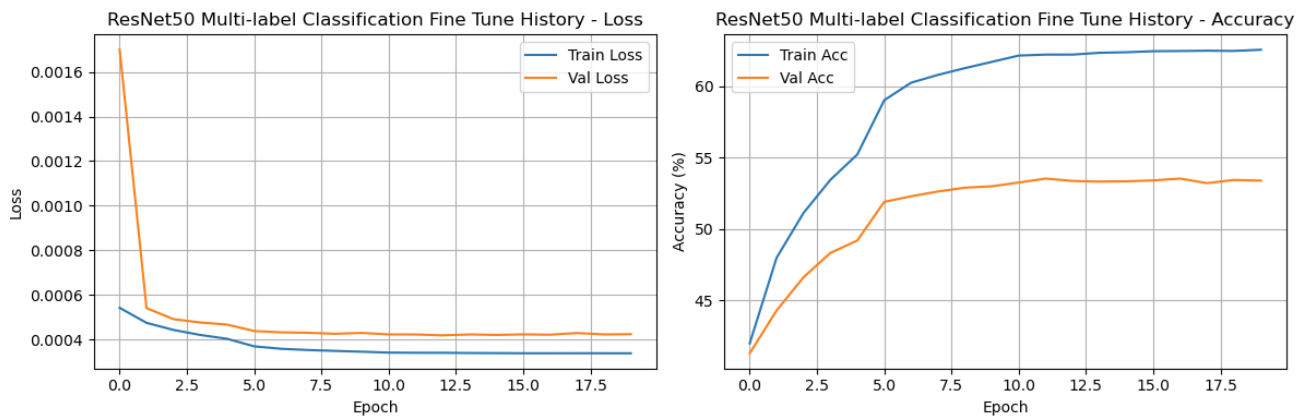
\includegraphics[width=1\linewidth]{ResNet50_fine_tune.png}
    \caption{Fine tune result of ResNet50 with single-plant training images}
\end{figure}

We were able to bring the validation accuracy from 40\% up to 54\%, after which the model performance seems to plateau (Figure 3). The fine tuning accuracy did not look very encouraging, which might be due to the 7.8k classes, many of which might be close species bearing high resemblance. 
With the fine tuned ResNet50 baseline model, we explored the impact of tiling stategy on zero-shot prediction performance. As shown in Figure 4, the model prediction was very poor when no tiling (\textit{i.e.}, tiling of 1x1) was performed, implying that little information could be used by the model due to the severe down-scaling of the high-resolution quadrat images. We then applied various tiling configurations and made model inference on each of the tiles for one quadrat, followed by a simple aggregation step that pools all non-repeated predictions together. As we can see from Figure 4, tiling greatly improved the model performance. Even a small tiling setup like 3x3 improved the macro-averaged F1 score by 8$\sim$10 times. The 5x5, 7x7, and 9x9 configurations all significantly outperformed the 3x3 tiling, with the 5x5 tiling yielding the highest private F1 score at a threshold of 0.2 and 7x7 tiling yielding the highest public F1 score at a threshold of 0.4. Since we did not see any obvious improvement of 9x9 tiling over 7x7, we did not go beyond 9x9 tiling, such as 11x11.       

\begin{figure}[H]
    \centering
    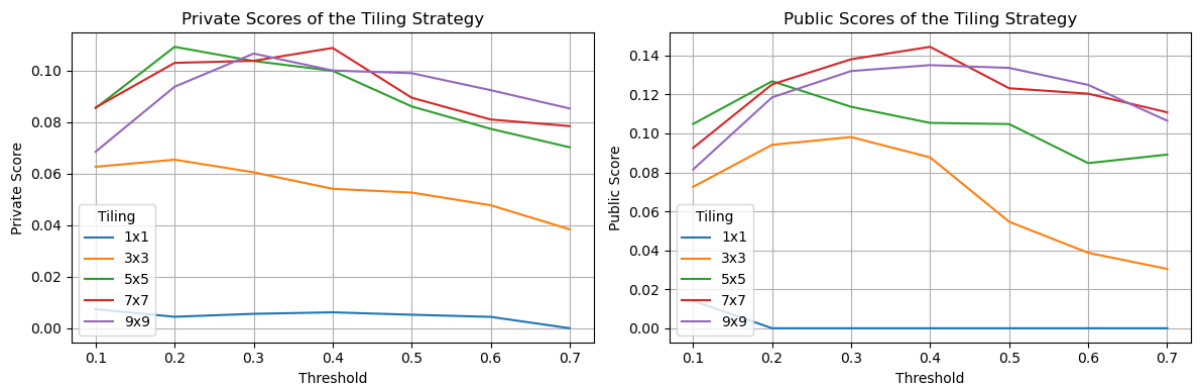
\includegraphics[width=1\linewidth]{ResNet50_tiling_ablation.png}
    \caption{Exploration of tiling configurations on ResNet50 model performance}
\end{figure}

Next, we explored the effect of voting and pooling on the baseline model performance. During the aggregation stage, we added a voting step that only accepts the predicted species labels with a certain frequency relative to the label with the highest count/frequency at the quadrat level. Different frequency ratios ($\in \{0.25, 0.50, 0.75\}$) were used as a cutoff during the prediction aggregation. Since the 5x5, 7x7, and 9x9 tiling configurations worked similarly well in the tiling ablation study, we kept all three tiling configurations while performing the voting exploration. As shown in Figure 5, adding a voting step brought the best F1 scores (both private and public) higher than without voting. 

\begin{figure}[H]
    \centering
    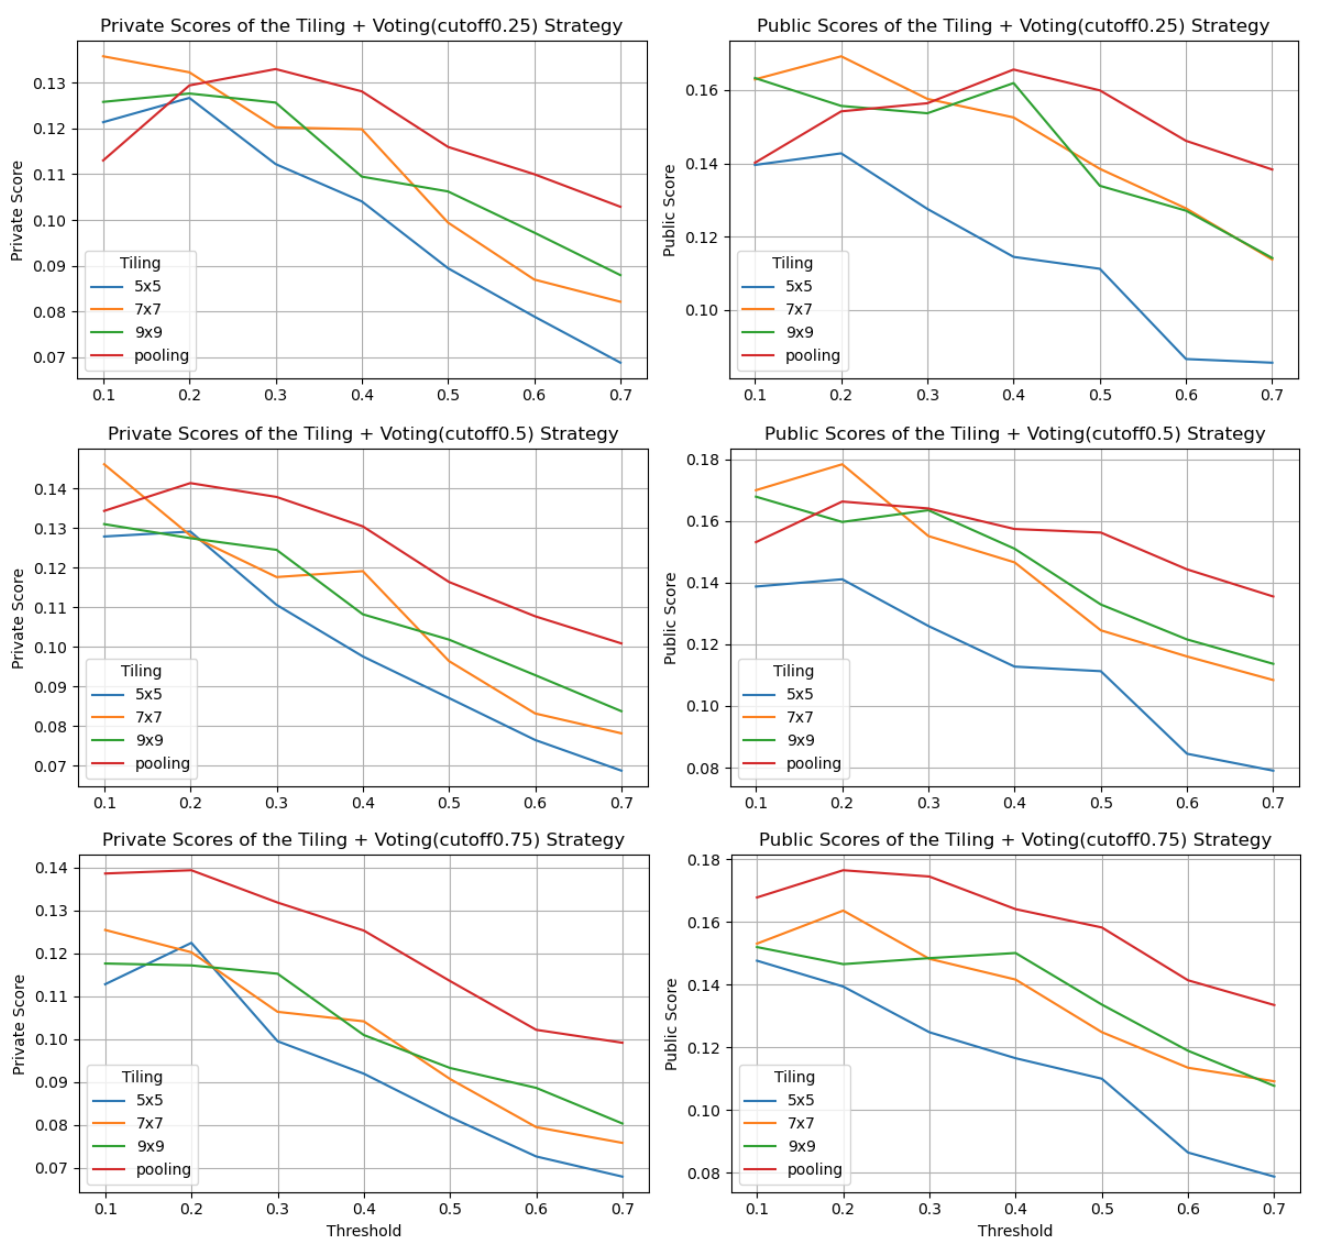
\includegraphics[width=1\linewidth]{ResNet50_voting_ablation.png}
    \caption{Exploration of voting on ResNet50 model performance}
\end{figure}

We also noticed that the best F1 scores were always generated with low thresholds from the multi-label classification step. This indicates that due to the large number of classes and the uncertainty the baseline model is facing, a relatively high threshold may not produce enough predictions whereas a low threshold may produce enough number of predictions but at the same time introduce a lot more false predictions. The introduction of voting effectively removes false positives from sufficient prediction candidates and thus presumably increases the precision. Therefore, we saw best F1 scores at lower thresholds, such as 0.1 and 0.2, across all voting cutoff values (Figure 5). Additionally, we found that the best F1 scores always came from the 7x7 tiling configuration, suggesting that 7x7 tiling or 49 tiles per quadrat provides the baseline ResNet50 with a generally optimal input resolution of each tile for the high-resolution quadrat images. Not surprisingly, 7x7 tiling gave the overall best private F1 score of 0.14604 and the overall best public F1 score of 0.1784 (Table 2).

Although voting clearly improves our baseline model performance presumably by removing false positive predictions, it remains unclear whether voting also simultaneously removes a considerable amount of true positives. To test this or to include as many true positives as possible, we conducted another ablation study on pooling, which pools together the voted predictions from 5x5, 7x7, and 9x9 tiling. As we can see from Figure 5, pooling (the red traces) significantly brought up the F1 scores for all of the predictions with a threshold greater than 0.3 and a voting cutoff of 0.25 or 0.5. In the case of voting at a cutoff of 0.75, pooling dramatically increased the prediction F1 scores regardless of the threshold. This result indicates that pooling improves the performance by bring together true positives across different model predictions (like ensemble), and that a high cutoff value is very stringent on prediction validity while the baseline model is also effective on capturing objects that are specific to their respective tiling.

Finally, the pooling results showed much less variation across the threshold range (Figure 5), indicating that pooling brings robustness to the model performance, making it less flexible or less dependent on the threshold setting during inference in this case. Figure 6 also supports the robustness of model performance introduced by pooling. As we can see that pooling results have very low variability across the threshold range and low sensitivity to the cutoff values for voting. 

\begin{figure}[H]
    \centering
    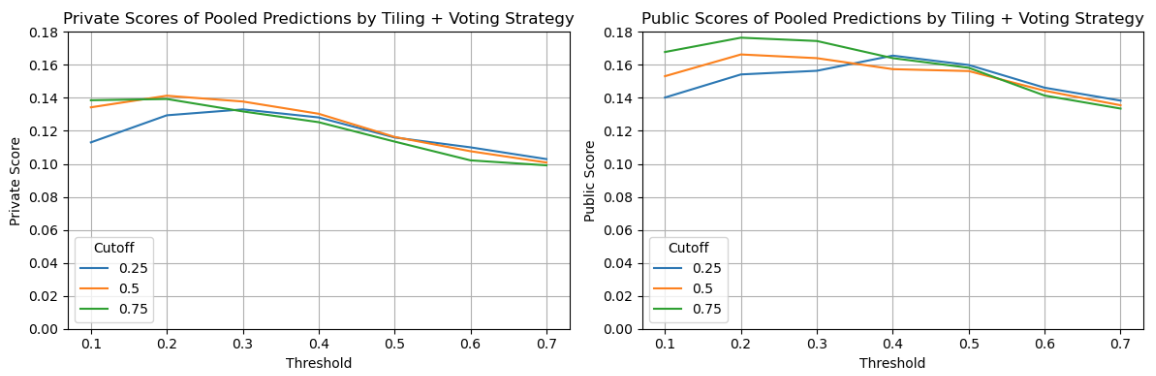
\includegraphics[width=1\linewidth]{ResNet50_pooling_ablation.png}
    \caption{Pooling of different ResNet50 model predictions}
\end{figure}


\subsection{ViTD2PC24All}

To test retrieval without training the model, we extract frozen [CLS] embeddings from the pre-trained ViTD2PC24All model provided by the PlantCLEF 2025 organizers for single plant images. Next, we create a FAISS index from these embeddings and for each tile of each quadrat, retrieve the $k=5$ nearest neighbors from our FAISS index. Finally, we obtain class predictions for the whole quadrat via voting. For these tests, the minimum number of votes - the amount needed to include the species in the predictions for the quadrat - was set to one.

The results of the grid size experiment are shown in the table below.

\begin{table}[H]
\centering
\caption{Grid size ablation on kNN}
\label{tab:baseline-dino}
\begin{tabular}{@{}ccc@{}}
\toprule
\textbf{Grid Size} & \textbf{Macro-F1 (Private)} & \textbf{Macro-F1 (Public)} \\ \midrule
3x3                & 0.14712                     & 0.16061                    \\
4x4                & 0.12922                     & 0.14406                    \\
5x5                & 0.10099                     & 0.11482                    \\ \bottomrule
\end{tabular}
\end{table}

As we can see, the 3x3 grid performs notably better than the 5x5 and 4x4 grids, confirming the results of many other contestants in the challenge.

We then tested the additional ablation methods from the ResNet50 study on the DinoV2 model. Here we looked at the effect of voting, pooling, and finally LoRA SSL. We observe results similar to those of the base ResNet model ablation study. In general, as we add tiling, voting, and finally pooling, the overall Macro F1 score increases. In the future, with the fully trained classification head, we can leverage these learned ablations to improve overall efficacy.


\section{Results}

\subsection{Ablation Results}

Here we have the results from our complete ablation study on both the ResNet50 baseline model and the ViT model before finetuning.

\begin{table}[H]
      \caption{Baseline Ablation Results}
        \label{tab:ablation}

      \begin{tabular}{lccc}
        \toprule
        \textbf{Model} & \textbf{Macro-F1 (private)} & \textbf{Macro-F1 (public)}\\
        \midrule
        Baseline (ResNet)  & 0.00738 & 0.01410 \\
        \-\hspace{0.2cm} Ablation: Grid Size & 0.10886 & 0.14443 \\
        \-\hspace{0.2cm} Ablation: Voting & 0.14604 & 0.17840 \\
        \-\hspace{0.2cm} Ablation: Pooling & 0.14129 & 0.17647 \\
        ViT (DinoV2)  & 0.01634 & 0.01723 \\
        \-\hspace{0.2cm} Ablation: Grid Size & 0.0852 & 0.06971 \\
        \-\hspace{0.2cm} Ablation: kNN voting & 0.09607 & 0.11804 \\
        \-\hspace{0.2cm} Ablation: Pooling & 0.12081 & 0.14523 \\
        %\-\hspace{0.2cm} Ablation: LoRA SSL & 0.15668 & 0.18754 \\
        %\textbf{Final ViT + Tiling} & \textbf{0.15668} & \textbf{0.18754} \\
        \bottomrule
      \end{tabular}
    \end{table}

\subsection{ViT Ablations}

To establish a robust baseline, we performed linear probing on the ViTD2PC24All model provided by the challenge organizers. A linear classification head was trained on the complete single-plant dataset for 15 epochs with a learning rate of 0.01, while the backbone weights remained frozen. We subsequently evaluated the inference performance across various spatial decomposition strategies, specifically analyzing the impact of grid tiling and multi-grid pooling. For the pooling experiments, we utilized a "union pooling" strategy, where the final prediction for a quadrat consists of the set union of all unique species predicted across individual tiles from different grid configurations. The best performing strategies are compared against the holistic baseline below, but the full ablation results are presented in Appendix Figures \ref{tab:baseline-dino_all} and \ref{tab:dino_pool_all}.

\begin{table}[H]
\centering
\caption{Ablation study of inference strategies for the DINOv2 baseline.}
\label{tab:dino_ablations}
\begin{tabular}{@{}ccc@{}}
\toprule
\textbf{Inference Strategy}  & \textbf{Configuration}     & \textbf{Best Macro-F1 (Private)} \\ \midrule
Holistic Baseline            & 1x1 Grid, Full Image       & 0.11524                          \\
Tiling                       & 3x4 Grid                   & \textbf{0.29368}                 \\
Multi-Grid Pooling           & 3x4 + 4x3 Grids            & 0.26823                          \\ \bottomrule
\end{tabular}
\end{table}

The results of this ablation study, presented in Table \ref{tab:dino_ablations}, indicate that decomposing the high-resolution quadrats into tiles significantly improves performance compared to the holistic approach (1×1), which likely suffers from the loss of fine-grained detail during resizing. In particular, while union pooling across multiple grid geometries offers a substantial improvement over the holistic baseline, it does not outperform the optimized single-grid tiling strategy (3×4). This suggests that for this specific dataset and model, the inclusion of additional, potentially suboptimal grid configurations introduces more false positives than true positives, thereby degrading the precision component of the F1 score.
\subsection{Self-Supervised Learning via Low-Rank Adaptation}

To address the domain shift between single-plant imagery and complex vegetation quadrats, we employ Low-Rank Adaptation (LoRA) \cite{hu2021loralowrankadaptationlarge}, a parameter-efficient fine-tuning technique. While originally pioneered for Large Language Models, LoRA has proven highly effective for adapting Vision Transformers (ViTs) to downstream tasks. In our implementation, we freeze the pre-trained DINOv2 backbone and inject trainable low-rank decomposition matrices into the query, key, and value (Q,K,V) projections of the self-attention layers. Targeting the attention mechanism allows the model to adapt its focus to the specific textural and structural patterns of the quadrat data without destructively interfering with the feature extraction capabilities of the pre-trained Feed-Forward Networks (FFNs). The specific hyperparameters used are detailed in Table \ref{tab:lora_config}.
\begin{table}[H]
\centering
\caption{LoRA hyperparameters}
\label{tab:lora_config}
\begin{tabular}{@{}cc@{}}
\toprule
\textbf{Hyperparameter} & \textbf{Value} \\ \midrule
Rank                    & 16             \\
Alpha                   & 16             \\
Dropout                 & 0.1            \\ \bottomrule
\end{tabular}
\end{table}

For the unsupervised domain adaptation phase, we implement the Simple Framework for Contrastive Learning of Visual Representations (SimCLR) \cite{chen2020simpleframeworkcontrastivelearning}. This approach utilizes a stochastic data augmentation pipeline—consisting of random resized crops, color jittering, and random horizontal flips—to generate two correlated views of each image in the unlabeled LUCAS dataset. We optimize the Normalized Temperature-scaled Cross Entropy (NT-Xent) loss, which encourages the model to maximize the cosine similarity between positive pairs (augmented views of the same image) while minimizing the similarity with negative pairs (all other images in the batch) in the latent space. This process enforces invariance to lighting and geometric transformations, effectively teaching the model to recognize consistent vegetation features across the pseudo-quadrats.

To evaluate the efficacy of the proposed domain adaptation strategy, we conducted a controlled comparison between the LoRA-based pipeline and the linear probing baseline under identical training constraints. The LoRA pipeline followed a two-stage process: self-supervised pre-training on the LUCAS dataset (50 epochs), followed by supervised fine-tuning on single-plant images (5 epochs).

Due to the substantial computational overhead of LoRA—which necessitates propagating gradients through the entire depth of the Transformer to update the injected adapters, unlike the frozen-backbone efficiency of linear probing—we restricted the training data to randomized subsets of 25,000 and 50,000 images. Table \ref{tab:lora_v_dino} presents the results of this comparison using the optimal 3×4 tiling strategy for inference.

\begin{table}[H] 
    \centering 
    \caption{Performance comparison between LoRA SSL and Baseline DINOv2 under identical data constraints (Private Macro-F1).} 
    \label{tab:lora_v_dino} 
    \begin{tabular}{@{}ccc@{}} 
        \toprule 
        \textbf{Training Set Size (N)} & \textbf{LoRA SSL (Ours)} & \textbf{Baseline DINOv2} \\ \midrule 
        25,000                         & \textbf{0.15668}         & 0.10495                  \\ 
        50,000                         & \textbf{0.23525}         & 0.13754                  \\ \bottomrule 
    \end{tabular}
\end{table}

The results demonstrate a marked performance advantage for the LoRA-adapted model. With a training budget of only 25,000 images, the LoRA approach achieves a Macro-F1 score of 0.15668, outperforming the baseline by approximately 49\%. This performance gap widens significantly as data availability increases; at 50,000 images, the LoRA model reaches an F1 score of 0.23525, representing a 71\% relative improvement over the baseline. This confirms that despite the higher computational cost per iteration, adapting the internal attention mechanisms via LoRA allows the model to learn domain-specific features that are critical for identifying plants within complex quadrats, a capability that linear probing on a frozen backbone fails to capture effectively.

\subsection{Grad-CAM Implementation}

To interpret the impact of self-supervised LoRA adaptation on the model's internal representations, we employed Gradient-weighted Class Activation Mapping (Grad-CAM) \cite{Selvaraju_2019}. Unlike Convolutional Neural Networks, where spatial features are preserved until global pooling, Vision Transformers aggregate information into a classification ([CLS]) token via self-attention mechanisms. Consequently, standard CNN hooking techniques are insufficient. Our implementation registers gradient hooks at the final LayerNorm (norm1) preceding the multi-head self-attention mechanism of the last Transformer block. This specific insertion point is critical: it captures the gradients of the patch tokens before they are weighted and aggregated into the [CLS] token, thereby allowing us to isolate the spatial contribution of specific image regions to the final classification.

\begin{figure}[H]
    \centering
    % First Subfigure
    \begin{subfigure}[]
        \centering
        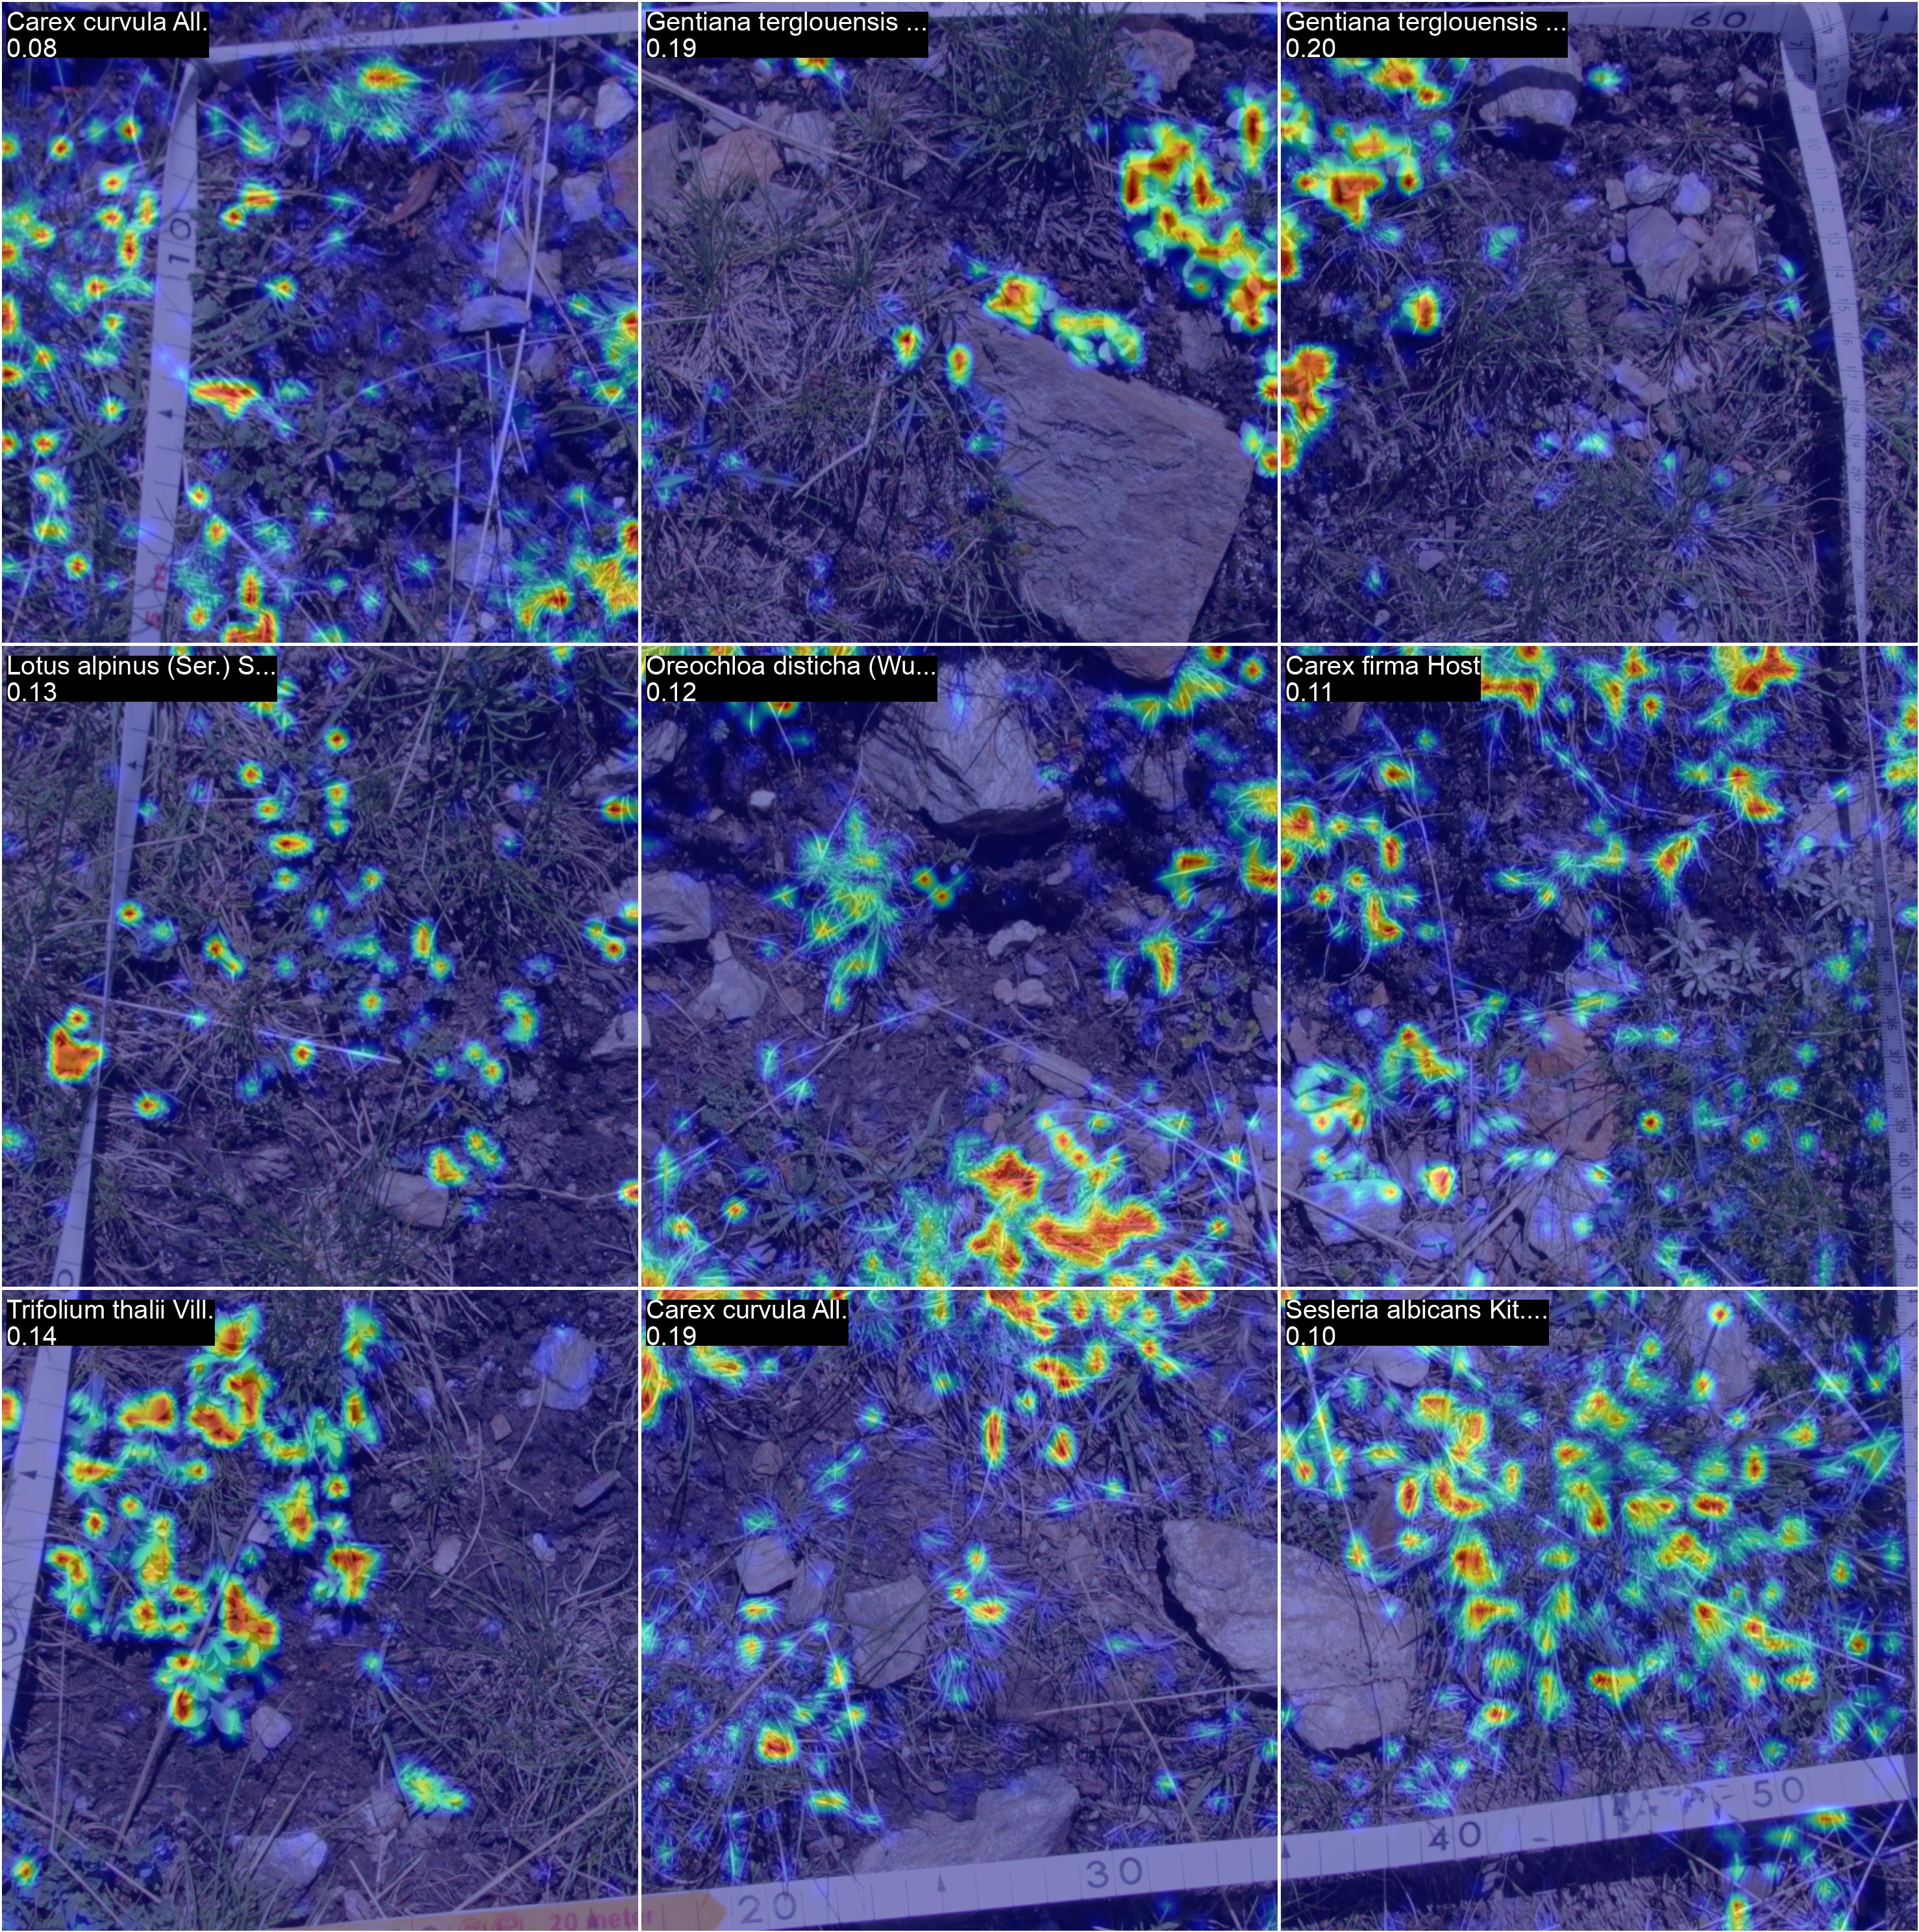
\includegraphics[width=.45\linewidth]{figures/gradcam_CBN-Pla-E1-20150723_baseline.jpg}
        \label{fig:sub1}
    \end{subfigure}
    \hfill % Adds flexible space between the images
    % Second Subfigure
    \begin{subfigure}[]
        \centering
        
\includegraphics[width=.45\linewidth]{figures/gradcam_CBN-Pla-E1-20150723_lora.jpg}
        \label{fig:sub2}
    \end{subfigure}
    
    \caption{GradCAM comparison of Baseline DINO (a) and LoRA SSL DINO trained on unlabeled quadrats (b).}
    \label{fig:side_by_side}
\end{figure}

Figure \ref{fig:side_by_side} presents a comparative visualization of these activation maps. The results indicate that the LoRA-adapted model captures the structural relationships and morphological boundaries of the plants more effectively than the baseline. This aligns with the hypothesis that self-supervised pre-training on the unannotated LUCAS dataset enables the model to internalize the dense, complex spatial distributions characteristic of vegetation quadrats—contextual features that are absent in the sparse, single-plant training distribution.

Notably, the visualization reveals that the LoRA model assigns high activation values to the measuring tape present in the image. This suggests that during the self-supervised contrastive learning phase, the model identified the measuring tape as a highly invariant feature across the LUCAS dataset. While this confirms the model's successful adaptation to the visual domain of the quadrats, it also highlights the risk of learning spurious correlations, where the model may rely on consistent anthropogenic artifacts rather than biological features for representation.

\section{Conclusion}
In this work, we presented a comprehensive pipeline for multi-label plant species identification, addressing the significant domain shift between sparse, single-plant training images and dense, high-resolution vegetation quadrats. Our ablation studies on a ResNet50 baseline demonstrated that spatial decomposition via tiling ($7\times7$) is critical for preserving fine-grained features, improving Macro-F1 scores by over an order of magnitude compared to holistic inference.

By transitioning to a Vision Transformer backbone (DINOv2), we achieved further performance gains. We demonstrated that simple linear probing on frozen backbones is insufficient for this task. Instead, our proposed Domain Adaptation strategy—utilizing Low-Rank Adaptation (LoRA) combined with self-supervised SimCLR pre-training on unlabeled quadrats—proved highly effective. This approach allowed the model to internalize the complex spatial and textural distributions of the test domain, yielding a 49\% performance improvement over the baseline when trained on limited data. Qualitative analysis via Grad-CAM further confirmed that the LoRA-adapted model captures structural plant boundaries more effectively than the baseline. Our optimal configuration, utilizing a $3\times4$ tiling strategy with a fine-tuned DINOv2 backbone, achieved a competitive private Macro-F1 score of 0.29368, underscoring the potential of parameter-efficient transfer learning in ecological monitoring applications.

\section{Future Research}

For further study, work should be done on the classification head and its implementations. It is not unreasonable to expect that, with the domain knowledge gained from the ResNet ablation studies, implementing Pooling/LoRA could make the model truly competitive with the top scores. As it stands, the 3x4 grid score of .29 is highly competitive. If the competition were held today, we would be in 12th place.

\section{Declaration on Generative AI}
During the preparation of this work, the author(s) used ChatGPT, GitHub Copilot, and Grammarly in order to: check grammar and spelling, paraphrase, and reword. After using this tool/service, the author(s)reviewed and edited the content as needed and take(s) full responsibility for the publication’s content.

\section{Individual Contributions}

John Michael Epperson mainly focused on the FAISS pipeline for extracting embeddings from the pre-trained DINOv2 model and making quadrat level predictions using k-nearest neighbors. Additionally, he implemented GradCAM and helped with the DINO and LoRA training and inference pipelines.

Patrick Foster focused on the dataset loading for single plant and full quadrat images. After John's KNN work, implemented training pipelines for DinoV2 and pooling.

Hai Liu primarily worked on the ResNet50 baseline and all its related training, fine-tuning, and ablation studies.

\bibliography{refs}
\bibliographystyle{unsrt}

\appendix

\section{ViT Ablations}

\begin{table}[H]
\centering
\caption{Grid size ablation on DINO ViT}
\label{tab:baseline-dino_all}
\small
\begin{tabular}{@{}ccc@{}}
\toprule
\textbf{Grid Size} & \textbf{Macro-F1 (Private)} & \textbf{Macro-F1 (Public)} \\ \midrule
3x3                & 0.27864                     & 0.26397                    \\
3x4                & 0.29368                     & 0.28049                    \\
4x4                & 0.27989                     & 0.25913                    \\
5x5                & 0.23912                     & 0.24488                    \\
7x7                & 0.17751                     & 0.19040                    \\ \bottomrule
\end{tabular}
\end{table}


\begin{table}[H]
\centering
\caption{DINO ViT Pooling Ablations}
\label{tab:dino_pool_all}
\begin{tabular}{@{}ccc@{}}
\toprule
\textbf{Pool}   & \textbf{Macro-F1 (Private)} & \textbf{Macro-F1 (Public)} \\ \midrule
3x3 + 4x4 + 5x5 & 0.21483                     & 0.22767                    \\
3x4 + 4x3       & 0.26823                     & 0.25575                    \\
6x6 + 7x7 + 8x8 & 0.12408                     & 0.14145                    \\
7x7 + 8x8 + 9x9 & 0.10228                     & 0.12245                    \\
2x2 + 4x4 + 6x6 & 0.18476                     & 0.20208                    \\
3x3 + 5x5 + 7x7 & 0.16297                     & 0.17904                    \\ \bottomrule
\end{tabular}
\end{table}

\end{document}
